\documentclass[12pt]{exam}

\usepackage{amssymb,amsfonts,amsmath}
\usepackage[letterpaper,margin=1in]{geometry}
\usepackage{graphicx}
\usepackage[numbered]{matlab-prettifier}
\usepackage{adjustbox}
\usepackage[T1]{fontenc}
\usepackage{mathtools}
\usepackage{color}
\usepackage{float}
\usepackage{bbold}

\DeclarePairedDelimiter{\abs}{\lvert}{\rvert}
\DeclarePairedDelimiter{\norm}{\lVert}{\rVert}

\renewcommand*{\vec}[1]{\boldsymbol{#1}}

\newcommand{\class}{Physics 306L}
\newcommand{\term}{Fall 2016}
\newcommand{\doctitle}{Lab Write-Up 10: Oscillators}

\parindent 0ex

\pagestyle{head}
\header{\bf \class}{\bf \doctitle\ - Page \thepage\ of \numpages}{\bf \term}
\headrule


\begin{document}
\framebox{\parbox{\dimexpr\linewidth-2\fboxsep-2\fboxrule}{
\begin{centering}
\textbf{Phase-shift Oscillator Values and Functions}\\
$R_1 =4.68 k\Omega, \quad R_2 =4.9 k\Omega,\quad R_3 = 4.7 k\Omega $\\
$C_1 = 9.9\text{nF}, \quad C_2 = 9.9\text{nF},\quad C_3 = 10 \text{nF}$\\
\textbf{DSA - Using op-am}\\
$R_a = 100.1 k\Omega, \quad R_b = 3.26M\Omega$\\
\textbf{Function Used}\\
$G = \frac{V_{out}}{V_{in}} = \left(\frac{V_{out}}{V_2}\right)  \left(\frac{V_{2}}{V_1}\right)  \left(\frac{V_{1}}{V_in}\right) $\\
\end{centering}
\begin{figure}[H]
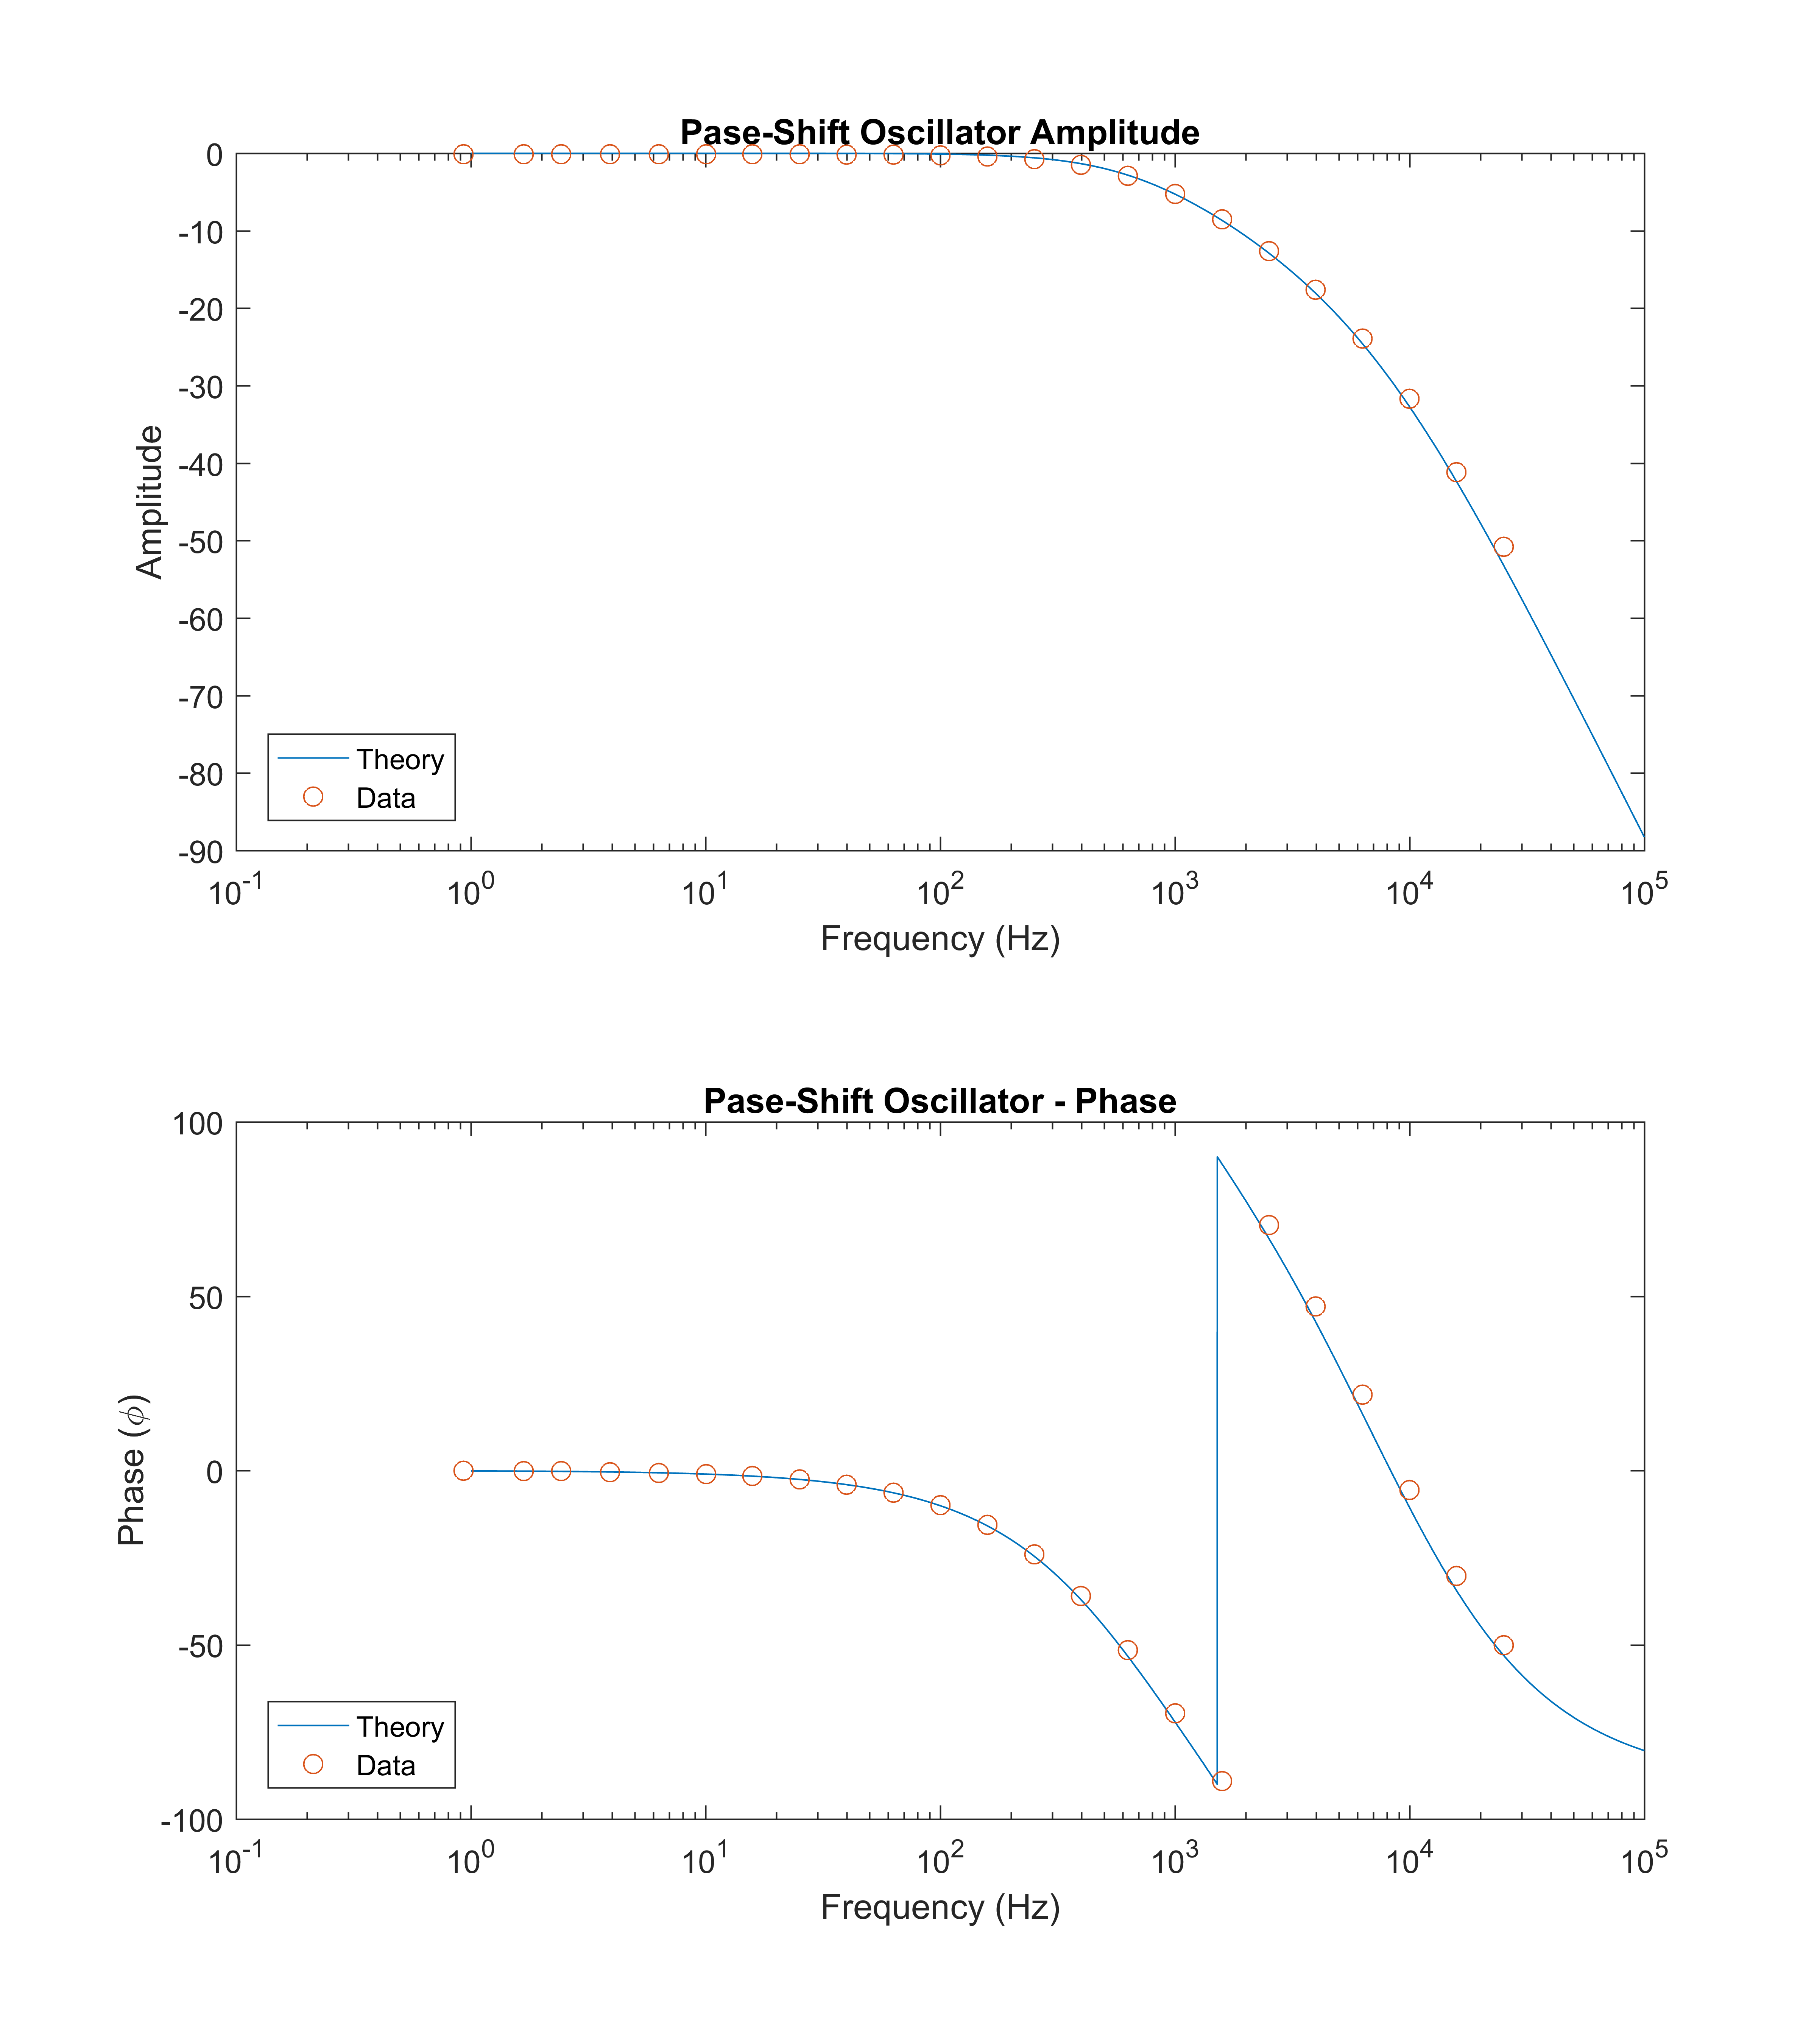
\includegraphics[width=\textwidth,keepaspectratio=true]{pso.png}
\end{figure}
}}


\framebox{\parbox{\dimexpr\linewidth-2\fboxsep-2\fboxrule}{
\begin{centering}
\textbf{Buffered Phase-shift Oscillator Values and Functions}\\
$R_1 =4.68 k\Omega, \quad R_2 =4.9 k\Omega,\quad R_3 = 4.7 k\Omega $\\
$C_1 = 9.9\text{nF}, \quad C_2 = 9.9\text{nF},\quad C_3 = 10 \text{nF}$\\
\textbf{DSA - Using op-am}\\
$R_a = 100.1 k\Omega, \quad R_b = 1.2M\Omega$\\
\textbf{Function Used}\\
$G = \frac{V_{out}}{V_{in}}  = \left(\frac{1}{1+ j\omega R_1 C_1}\right)  \left(\frac{1}{1+ j\omega R_2 C_2}\right)  \left(\frac{1}{1+ j\omega R_3 C_3}\right) $\\
\end{centering}
\begin{figure}[H]
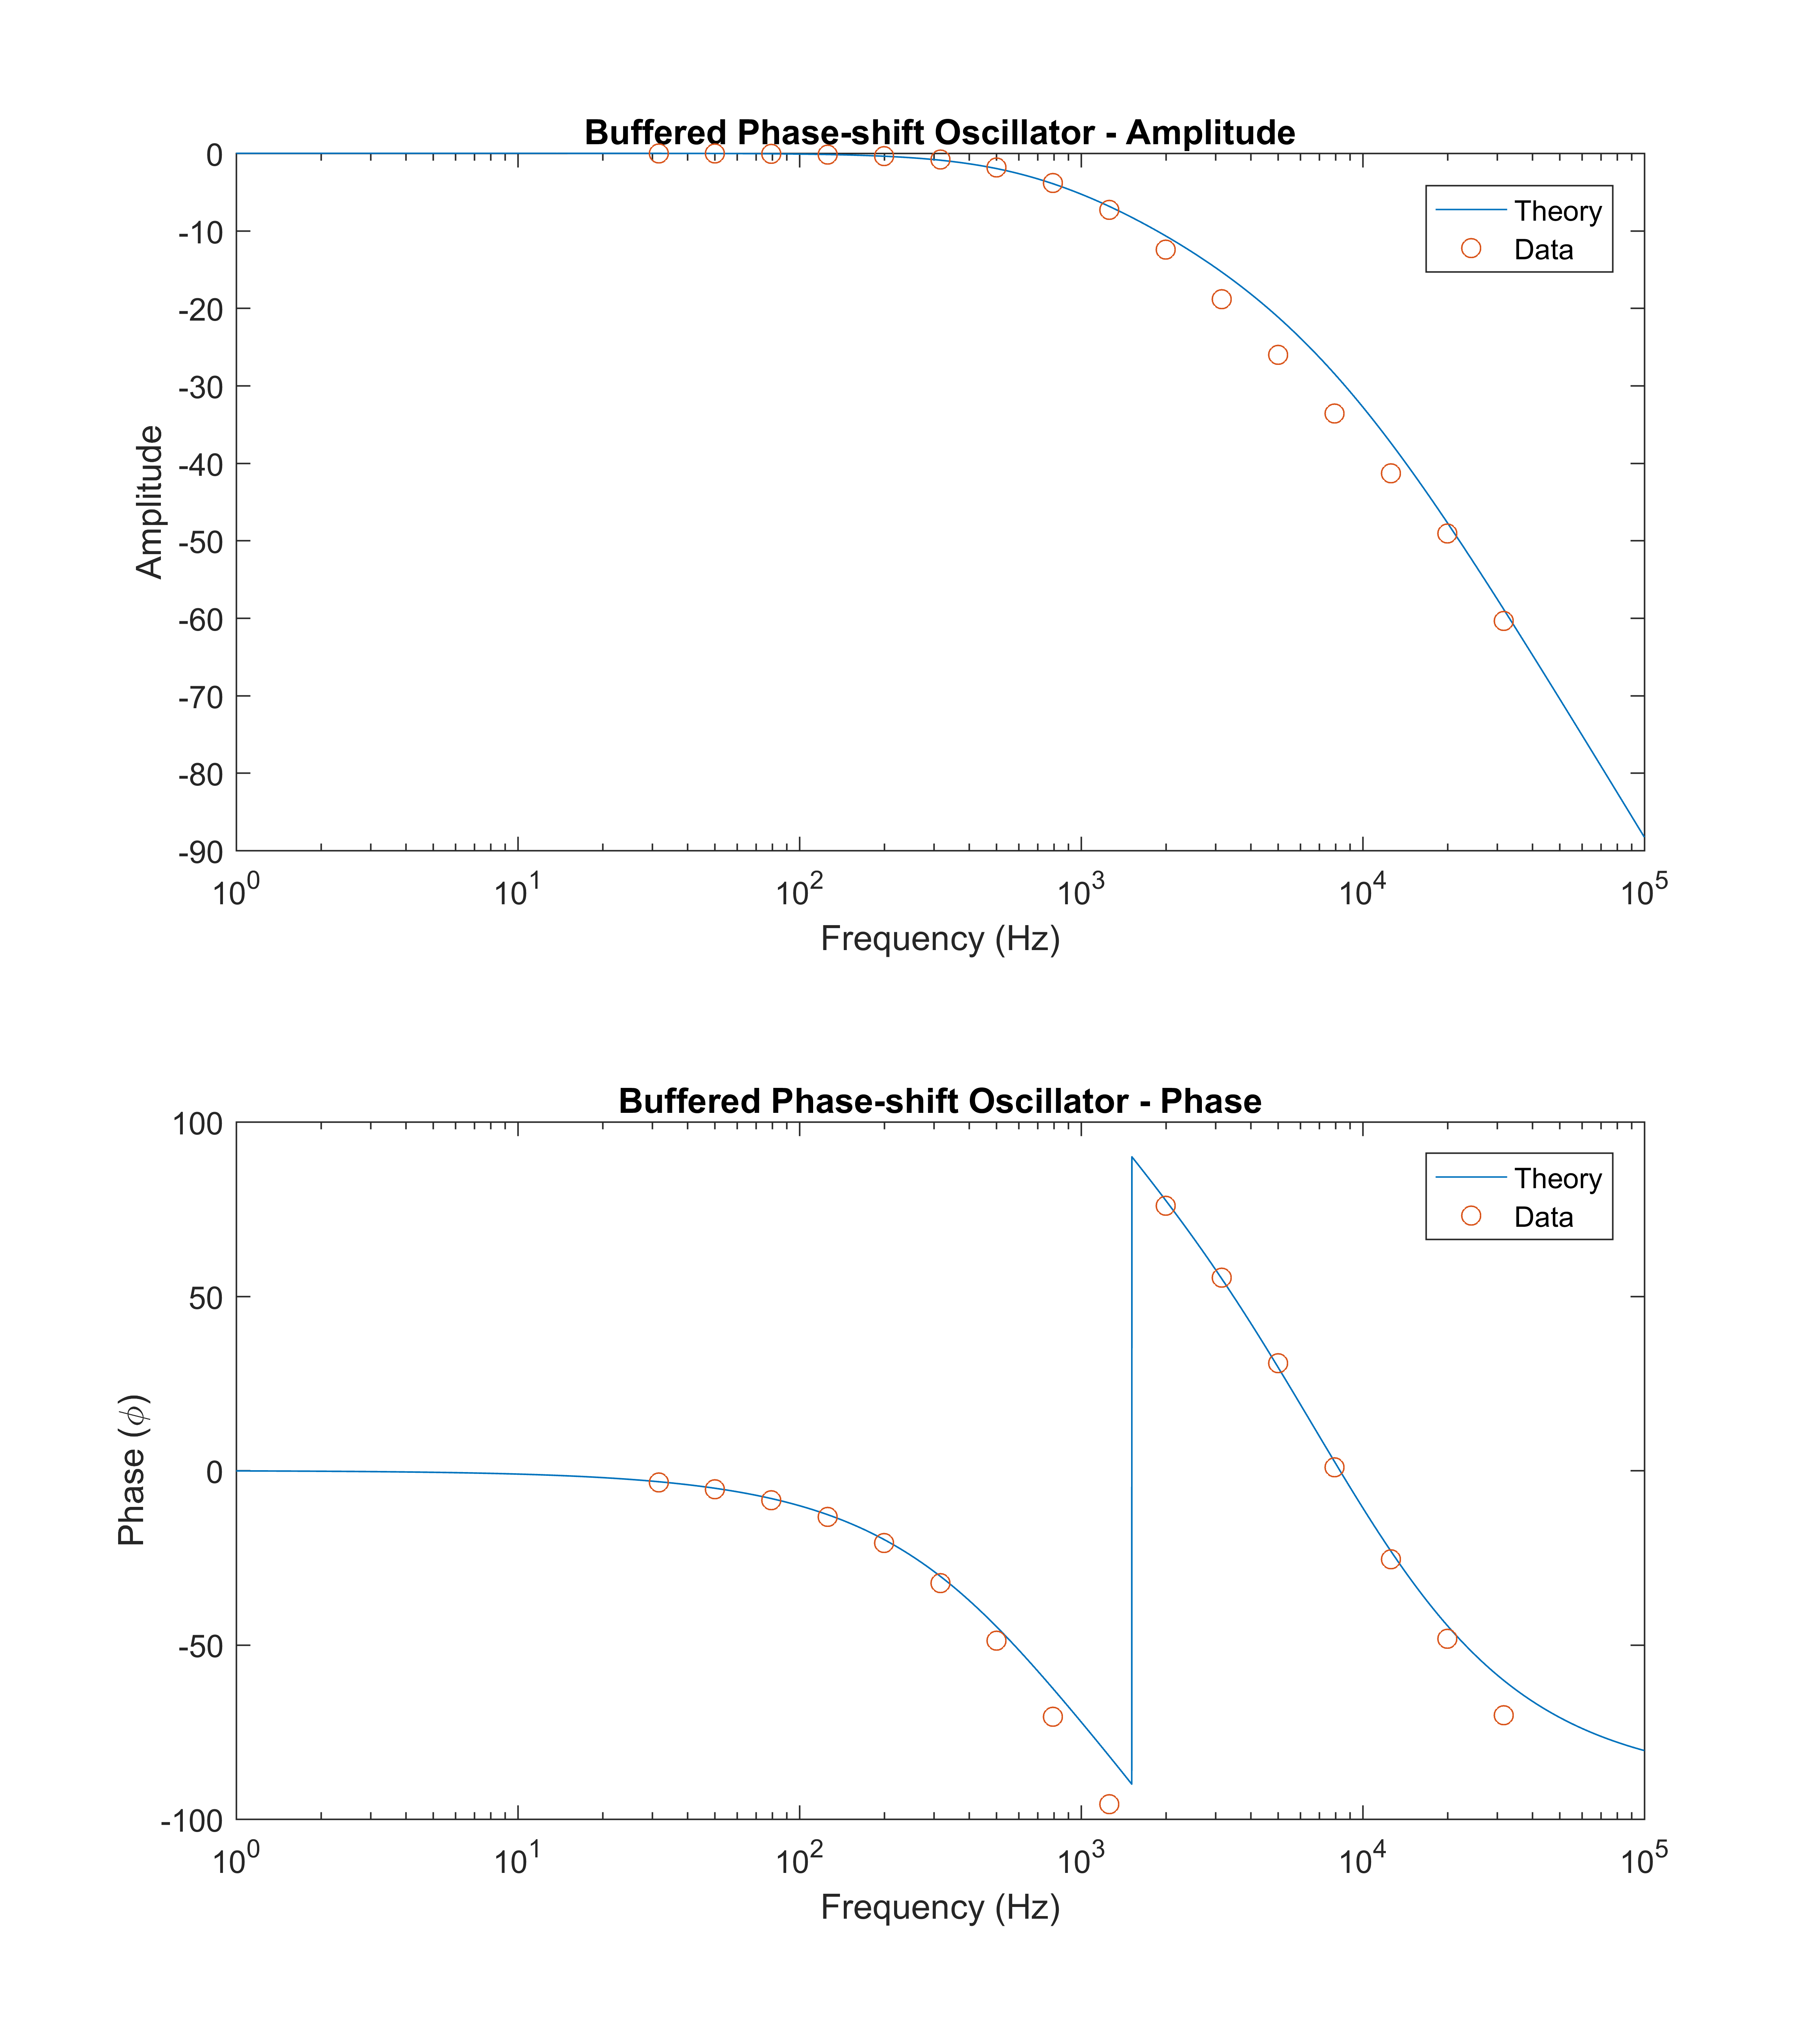
\includegraphics[width=\textwidth,keepaspectratio=true]{buffered.png}
\end{figure}
}}


\framebox{\parbox{\dimexpr\linewidth-2\fboxsep-2\fboxrule}{
\begin{centering}
\textbf{DSA - Plots}\\
\end{centering}

\begin{figure}[H]
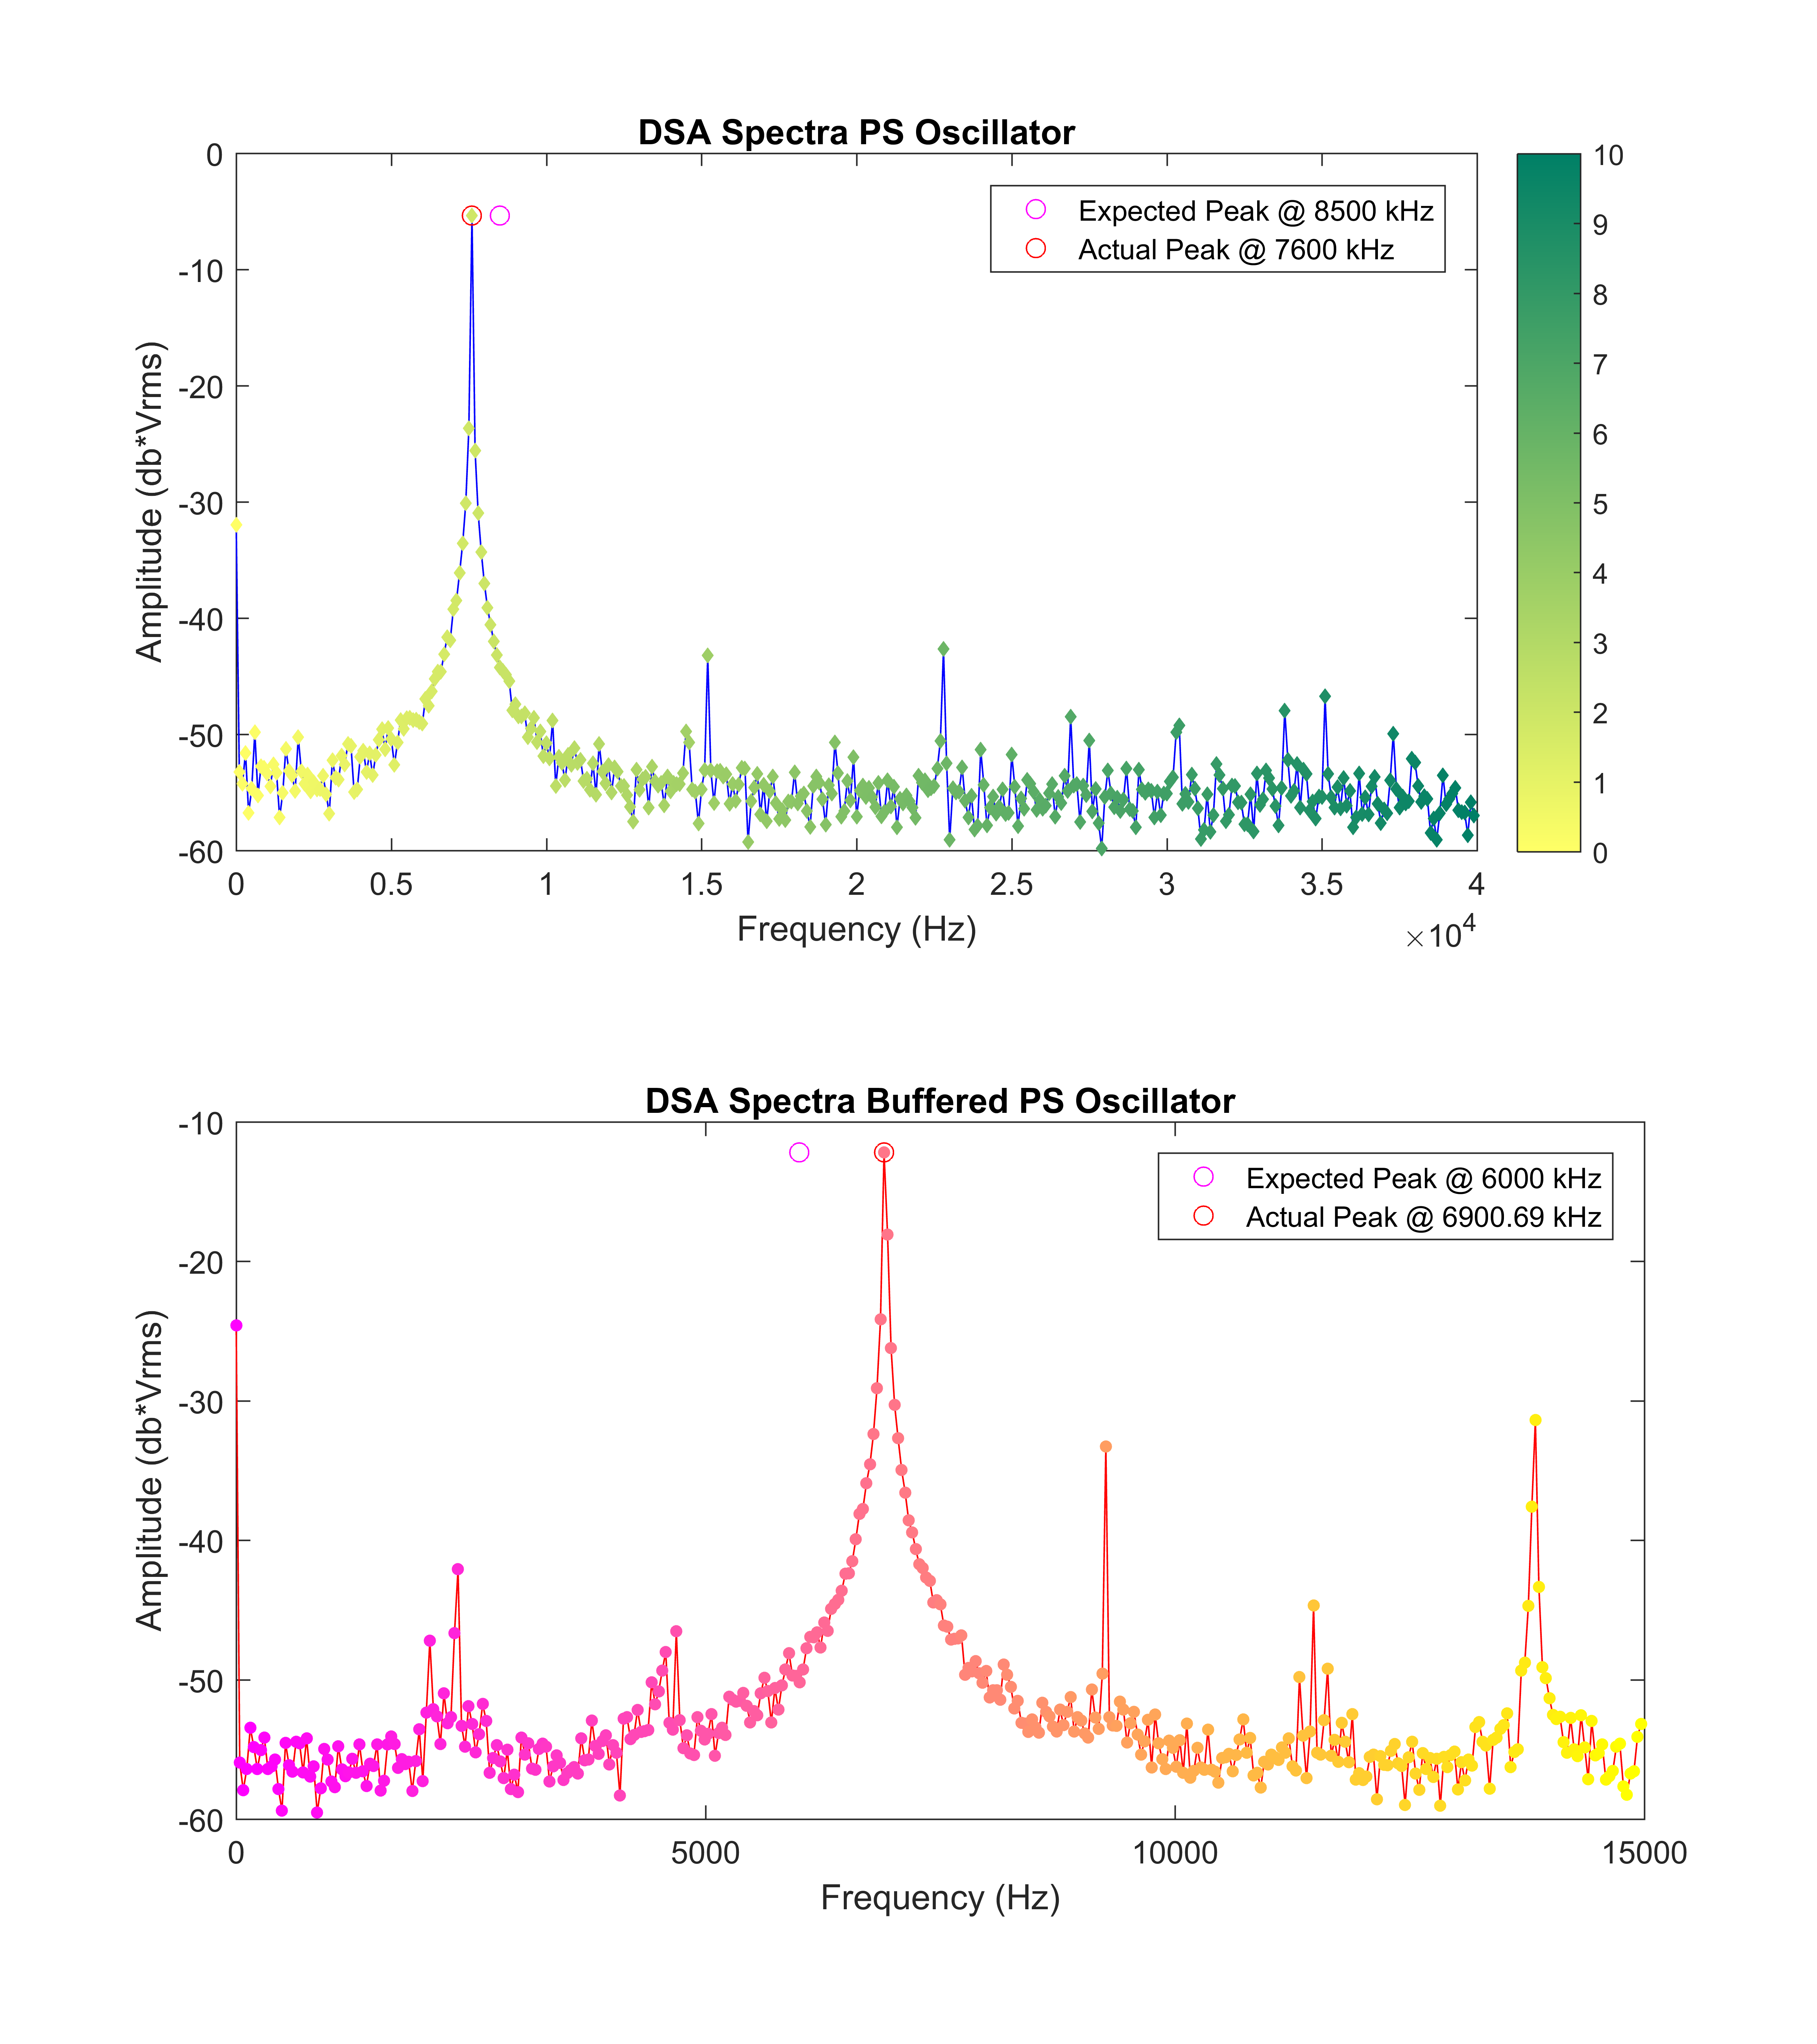
\includegraphics[width=\textwidth,keepaspectratio=true]{DSA.png}
\end{figure}
}}


\end{document}
